\documentclass[a4paper,11pt]{article}
\usepackage[spanish, activeacute]{babel}

\addtolength{\topmargin}{-80pt}
\addtolength{\textwidth}{170pt}
\addtolength{\textheight}{145pt}
\addtolength{\oddsidemargin}{-80pt}

\usepackage{graphicx} % para incluir graficos
\usepackage{amsmath} 
\usepackage{amsthm} % para escribir teoremas lindos
\usepackage{amsfonts} % para tener el simbolo de los numeros reales
\usepackage{color}  % colores de las fuentes

\theoremstyle{definition} \newtheorem{axiom}{Axioma}

\begin{document}
\newcommand{\Nat}{\mathbb{N}}
\newcommand{\cita}{\textcolor{red}{cita}}
\newcommand{\red}[1]{\textcolor{red}{#1}}

\tableofcontents

\section{Introducci\'on y objetivos}
Hacia fines del siglo XIX y principios del siglo XX (\alert{revisar}), con el prop'osito de estudiar la estructura interna de una pieza musical, 
Heinrich Schenker elabor'o un m'etodo de an'alisis musical conocido como \texttt{an'alisis schenkeriano}.
Esta estructura es descripta por el autor en t'erminos de \texttt{reducciones}. Una reducci'on permite especificar que una cierta nota dentro de un grupo es la fundamental, 
y que todo el resto es una \texttt{elaboraci'on} de esta. Dado que esta relaci'on de reducci'on/elaboraci'on se puede aplicar recursivamente, naturalmente emerge una relaci'on 
jer'arquica entre las notas de una pieza musical.  En esta jerarqu'ia, el nivel m'as bajo es lo que se encuentra escrito en la partitura, y a medida que se sube de nivel se 
encuentra la misma pieza musical, pero carente de elaboraciones. A continuaci'on se excibe un ejemplo de dicho an'alisis:


\begin{figure}[h]
\begin{center}
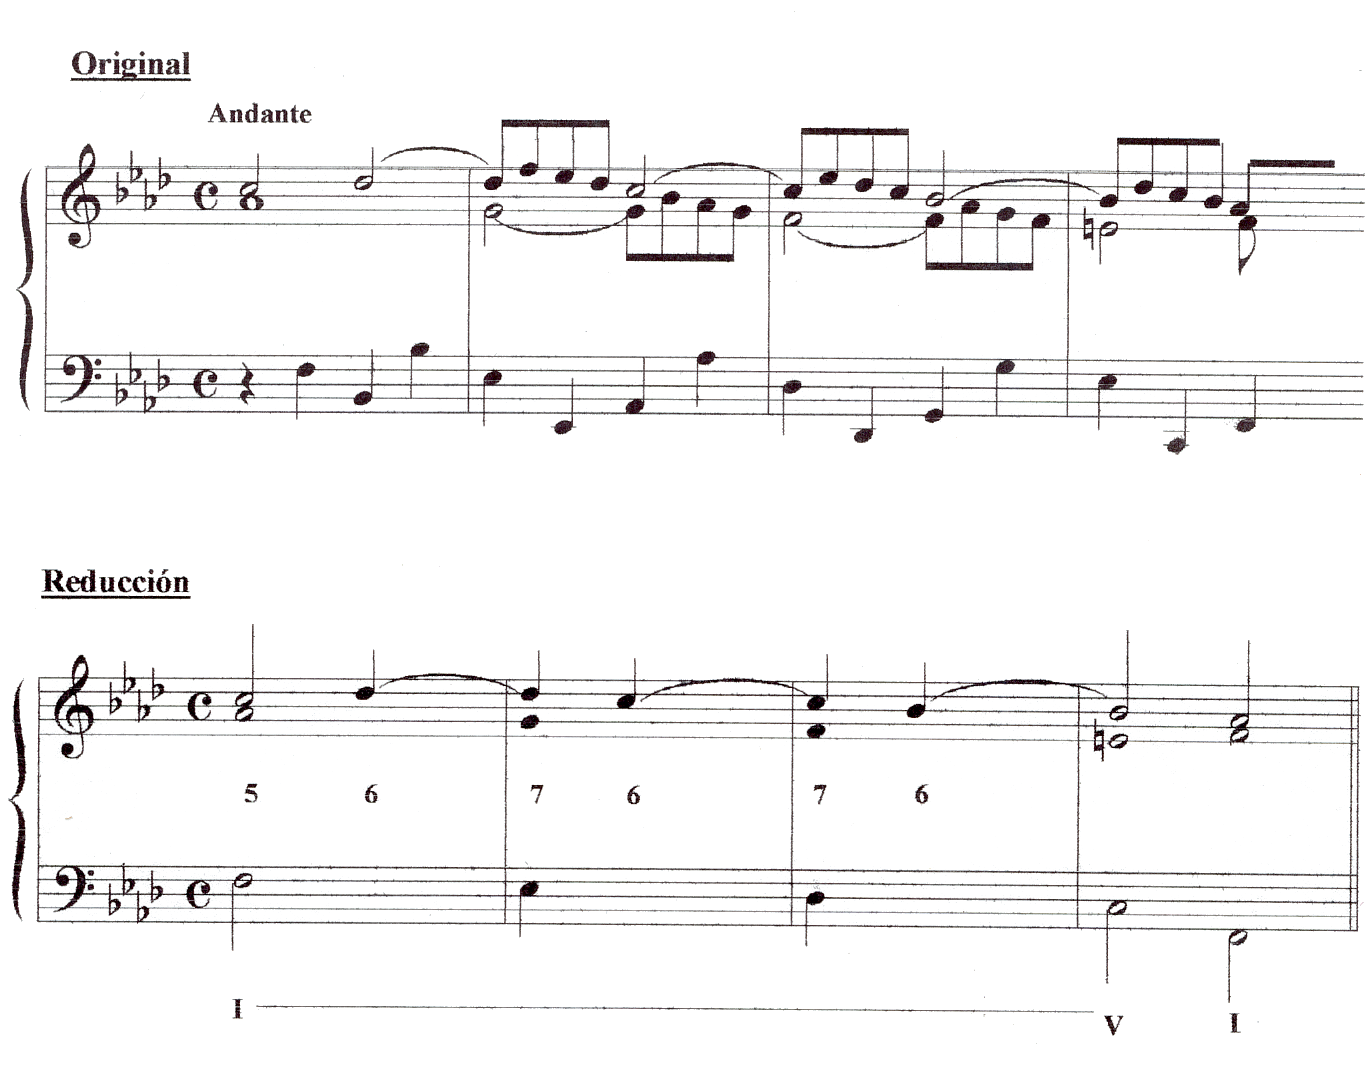
\includegraphics[width=12cm]{images/schenkerian_example.png}
\newline \alert{poner una imagen mas copada}
\end{center}
\end{figure}

En esta figura, los sucesivos pentagramas muestran relaciones de reducci'on, as'i simplificando el tema con el objeto de llevarlo a una representaci'on mas concreta.

El parecido de este tipo de relaciones con las relaci'ones utilizadas por Noam Chomsky para analizar el lenguaje natural es notable. 
Si bien en la teor'ia de Chomsky las relaciones son relaciones del tipo ``es un'', y en la teor'ia de Schenker son del tipo ``es una elaboraci'on de'', 
estas se enmarcan matem'aticamente en el mismo lugar.  

En 1983, el m'usico Fred Lerdahl y el ling\"uista Ray Jackendoff publicaron el libro 
\texttt{A Generative Theory of Tonal Music}(GTTM) donde proponen una gram'atica para analizar la m'usica t'erminos parecidos a los de Schenker. 
Lo hace interesante a este trabajo es el fundamento que se le da a la elecci'on de las reglas de la gram'atica, puesto que analizan la teor'ia 
schenkeriana en t'erminos cognitivos.  

El objetivo del trabajo de Lerdahl y Jackendoff es principalmente tener un modelo que sea capaz de describir el proceso mediante el cual se estructura la percepci'on de la m'usica. 
Este modelo consiste en una serie de reglas de preferencia. Cada regla tiene asociado un predicado booleano $P$ y un valor de preferencia $v$, 
de modo que si el predicado booleano es verdadero, entonces aportan $v$ unidades a la preferencia de una cierta acci'on interpretativa. Para ejemplificar, a continuaci'on se cita
una regla de preferencia de los autores. Esta regla es una de las reglas asociadas a lo que los autores llaman agrupamiento, que b'asicamente consiste en agrupar notas que tienen
significancia de frase\footnote{M'as adelante se explicar'a esto con mayor detalle}.
\newline

\begin{center}
\texttt{GPR 1} Evite fuertemente grupos que contengan solamente un evento.
\end{center}

En este caso, el predicado booleano es aquel que es verdadero solamente con grupos de cardinalidad uno, y el valor de preferencia es fuertemente negativo a la acci'on interpretativa
de decidir que el grupo en cuesti'on debe contener 'unicamente al evento que contiene. Como esta, los autores exiben un gran conjunto de reglas que luego validan experimentalmente. 

Si bien un modelo de este tipo es generativo en el sentido de que podr'ia ser utilizado por una computadora tanto para analizar una pieza musical como para 
\texttt{generar} una nueva, es importante notar que este no es su objetivo. 
Puede verse claramente como la regla \emph{GPR 1} si bien es suficientemente rigurosa como para luego poder corroborarla emp'iricamente, no lo es como para construir un 
programa que haga un an'alisis utilizando esta regla: es necesario determinar el valor de preferencia y aprender las relaci'ones entre los distintos valores de preferencia para luego 
tomar una desici'on.  

De esta forma se discrimina entre \texttt{modelos generativos}, que son aquellos que eventualmente podr'ian utilizarse para generar aquello que explican, y 
\texttt{modelos de 'indole generativo} que fueron hechos con el objeto de generar aquello que explican.  El hecho de que sea necesario definir expl'icitamente los valores de preferencias
sumado a que este modelo no es de 'indole generativo plantea el interrogante de si realmente este enfoque es el adecuado para para modelar la cognici'on musical con aprendizaje 
autom'atico. 

De este modo, el objetivo de este trabajo es utilizar el conocimiento generado por trabajos como el de Lerdahl y Jackendoff como medio para establecer propiedades que un modelo de 
'indole generarivo deber'ia cumplir. Teniendo estas propiedades, luego es posible construir un modelo desvinculado con la idea de gram'atica, pero que respete 
ciertos criterios fundamentales. Si se logra conseguir un modelo de estas caracter'isticas se podr'an validar emp'iricamente los criterios en base a los que el modelo fue construido 
(y por lo tanto las teor'ias cognitivas motivaron los criterios) a trav'es de analizar las piezas musicales generadas por el modelo.

Para poder avanzar en pos del objetivo recien planteado, es necesario primero sentar un vocabulario para luego poder contextualizarlo. De esta forma, las siguientes dos
secci'ones hablaran sobre background. Luego se har'a un breve resumen sobre el estado del arte en este tema, para luego abordar el trabajo en concreto de esta tesis.


\section{Objetivos}

\section{Fundamentos cognitivos y musicales}
\label{sec_cogn_bg}
Principalmente, la m'usica tiene dos grandes componentes: la del \texttt{tiempo} y la de la 
\texttt{altura}. La dimensi\'on del tiempo se refiere a las duraci\'ones de los distintos eventos que 
ocurren en una pieza musical. Por otro lado, la altura se refiere a la percepci\'on de las distintas notas que ocurren 
en un tema.es Es importante notar la diferencia entre la altura de una nota y la frecuencia de la misma; la altura refiere
a la percepci'on de una frecuencia.

Si bien estas dos dimensiones se presentan por separado, de ninguna manera son independientes. Ser'an abordadas de esta forma 
para facilitar una primera descripci'on. De ser necesario, posteriormente se elaborar'an los conceptos que refieran a las interacciones entre 
estas dos componentes. 

\subsection{La tensi\'on y lo esperable}
\label{subsec_tension}
\begin{itemize}
  \item 

\end{itemize}
\comment{aca voy a hablar sobre la relacion que hay entre la tension y lo esperable, definiendo como esperable a un evento en un cierto contexto, luego voy a distinguir entre
dos tipos de contextos: el horizontal y el vertical. El contexto horizontal tiene que ver con patrones en el tiempo, y el vertical con relaci'ones armonicas en un cierto
instante. Esto despues lo voy a usar para los modelos de la ritmica (solo usa contexto horizontal) y de la melodia (usa los dos contextos y arma un modelo conjunto)}


\subsection{El tiempo es racional: el concepto de \emph{beat}}
\comment{Esto no lo borro solo porque me costo escribirlo, pero creo que aca no pincha ni corta }\newline
En su libro, Lerdahl y Jackendoff(\cita) hacen una distinci'on entre dos estructuras que ocurren en simultaneidad en la m'usica tonal:
La estructura \emph{m'etrica} y la estructura del \emph{agrupamiento}\footnote{\emph{meter} y \emph{grouping} en ingl'es}. 
Esta distinci'on en t'erminos generales coincide con clasificaciones de otros autores (\alert{citas muchas!}), se toma la version de Lerdahl y Jackendoff 
por ser esta m'as computacional.
La estructura del agrupamiento hace referencia a la organizaci'on de una pieza musical en unidades que pueden ser motivos, frases, secciones, etc. 
Cada una de estas unidades, es denominada por los autores \emph{grupo}. Asimismo, el oyente infiere una estructura regular de pulsos. 
Algunos pulsos son m'as fuertes que otros, determinando lo que los autores definen como la estructura m'etrica. 
Para ponerlo en concreto pensar la estructura como la forma en la que un director de orquesta mueve su batuta. 
En lo subsiguiente se utilizar'an los t'erminos pulso y \emph{beat} como sin'onimos intercambiables.

Ambas estructuras tienen son jer'arquicas, en el sentido de que existen sub-estructuras a distintos niveles, y que las sub-estructuras de niveles superiores 
incluyen por completo a las de nivel inferior\footnote{Para una definici'on mas formal de la jerarqu'ia referirse a \cita}. De esta forma, una secci'on
de una pieza musical estar'a formada por una sucesi'on de frases. Estas frases s'olo pertenecer'an a esa secci'on, sin embargo, esto no quiere decir
que no se pueda repetir una frase en dos secciones distitnas, puesto que cada una pertenecer'a a una sola secci'on. 
Esto mismo ocurre con la estructura m'etrica; existen distintos niveles de beats dados por el tiempo que ocurre entre dos pulsos sucesivos. De esta forma, al 
ocurrir estos en tiempos regulares, s'olo hace falta saber cual es la distancia entre cualquier par de beats consecutivos para referirse a ese nivel. 

La organizaci'on jer'arquica de la m'usica no es una teor'ia solo postulada por Lerdahl y Jackendoff; Cooper y Meyer(\cita) plantean una teor'ia similar en
estos t'erminos, Kramer(\cita) si bien no habla directamente de una jerarqu'ia, propone que tienen un rol 
estructurante\footnote{\alert{tengo que leer m'as, as'i se mejor de lo que hablan estos dos muchachos}}. 

Un nivel de especial inter'es, es el denominado \emph{tactus}, que b'asicamente es el marcado por el director de orquesta al mover su batuta. 
El tactus tambi'en es la distancia entre los pulsos que el oyente marca cuando mueve el pie y est'a relacionado con el baile. 

Es importante notar que esta estructura es ambigua, en el sentido de que que muchas veces no existe un 'unico an'alisis de una pieza musical 
en una estructura m'etrica y de agrupamiento.


\subsection{Acentuaci\'on}
Una car'acteristica de la m'usica, tambi'en compartida con el habla, es que un mismo evento no es percibido de la misma forma seg'un
el contexto en el que ocurre. Hay varios factores que afectan el contexto, y uno de ellos es la \texttt{acentuaci\'on}. 

Un evento musical es escuchado como acentuado si es enfatizado de alg\'una forma. Lerdahl y Jackendoff(\cita) distinguen tres tipos de 
acentos: los acentos fenom'enico \footnote{\alert{se que no es esta la traducci\'on, como se dice en espa~nol?}}, estructurales y m'etricos.
Un acento fenomenal es cualquier evento que de 'enfasis o estress a un momento en la pieza musical. \alert{Que ejemplos doy? esto lo va a 
leer gente que \emph{no sabe} musica}. Los acentos estructurales son puntos de apoyo para finalizar una parte o una frase. 
Por 'ultimo, los acentos m'etricos son aquellos beats relativamente fuertes dentro del contexto m'etrico donde suceden.

Kramer(\cita) tambi'en reconoce tres tipos distintos de acentos, llamados \emph{m'etrico}, \emph{stress} y \emph{r'itmico}. Esta categorizaci'on
es equivalente a la dada por Lerdahl y Jackendoff.

Meyer(\cita) no elabora\footnote{checkear que sea realmente asi} una taxonom'ia de acentos. Su inter'es no est'a en saber \emph{qu'e} hace
que un pulso est'e acentuado sino \emph{c'omo} opera un pulso acentuado en terminos de estructura r'itmica. En estos t'erminos distingue
que los pulsos acentuados son de alguna forma el punto de foco donde los beats circundantes se agrupan. 

Es importante notar que este tipo de categorizaciones no son excluyentes, es decir, un beat puede tener m'as de un tipo de acento al mismo tiempo.
Para ejemplificar, dentro de la teor'ia de Lerdahl y Jackendoff se describe el proceso cognitivo por el cual se infieren los acentos m'etricos. Este
proceso consiste en que el oyente utiliza los acentos fenomenales y estructurales como pistas para extrapolar un patr'on regular de acentos m'etricos. 
Dentro de 'este contexto, no es la excepci'on, sino la regla que haya beats que son acentuados con un acento fenomenal y m'etrico al mismo tiempo.



\section{Background matem\'atico}
\label{sec:math_bg}
\subsection{Sobre estad\'istica bayesiana}
%Una de las decisiones sobre el alcance de este trabajo es que los modelos construidos ser'an entrenados s'olo con un tema por vez. 
%Esta decisi'on evita el problema de tener que combinar la informaci'on proporcionada por varias piezas musicales. Sin embargo, el precio que debe pagarse 
%es que para muchos modelos de los que se expondr'an no alcanza solamente con entrenar con una pieza musical, puesto que ciertas estimaciones 
%no ser'ian estad'isticamente significativas. 

Sup'ongase por un momento que uno desea estimar la probabilidad de que una cierta moneda caiga \emph{cara}. De contar con suficientes muestras, digamos 30, 
es posible calcular la frecuencia relativa de \emph{cara} dividiendo la cantidad de veces que se observ'o caer a la moneda en \emph{cara} por el total, 30. 
Sup'ongase ahora que por alguna raz'on se cuenta solamente con dos muestras y ambas resultaron en \emph{cara}. En este caso, la aproximaci'on frecuentista
estimar'ia que la probabilidad de \emph{cara} es $100\%$, estimaci'on que contradice el sentido com'un. 

Una soluci'on a este problema es adoptar una postura bayesiana y tener una creencia previa sobre las caracter'isticas del fen'omeno a modelar, 
y luego actualizar esta creencia previa con la evidencia observada. En este caso una creencia previa razonable ser'ia asumir que la moneda est'a balanceada
salvo que haya \emph{suficiente} evidencia que indique lo contrario. %De esta forma, si el modelo esta basado en una teor'ia cognitiva, se puede utilizar
%como creencia previa alg'un estudio donde se haya puesto a prueba esta teor'ia. 

Otra raz'on para utilizar creencias previas es para estimar distribuci'ones de probabilidades suaves, en el sentido de que no asignen valor $0$ a un evento 
por el s'olo hecho de no haberlo observado en la etapa de entrenamiento. 

Escribiendo esto matem'aticamente, sup'ongase que se cuenta con un mo\-delo parametrizado por un vector $\theta$. La creencia previa sobre el fen'omeno a modelar, b'asicamente estar'ia restringiendo \emph{a priori} qu'e par'ametros son m'as probables que otros. 
Esta informaci'on se codifica como una distribuci'on de probabilidades sobre $\theta$, $P(\theta)$. En el ejemplo de la moneda, $\theta$ 
tendr'a dos coordenadas, una para la probabilidad de que la moneda caiga en \emph{cara}, y otra para la probabilidad de que la moneda caiga \emph{seca}.
Dado que el vector $\theta$ expresa una distribuci'on de probabilidades, sus coordenadas deben sumar $1$. Es por esto que se puede considerar que en este caso en realidad hay un solo par'ametro.

Sup'ongase ahora que se cuenta con cierta evidencia de entrenamiento $x_1,\cdots,x_n$. Al entrenar el modelo, uno quisiera combinar la 
creencia previa dada por $P(\theta)$ junto con la evidencia dada por $x_1,\cdots,x_n$ en una distribuci'on \emph{a posteriori} sobre los par'ametros.
Utilizando la ley de Bayes y la ley de probabilidad total, es posible reescribir la distribuci'on a posteriori de $\theta$ en funci'on de su creencia previa y 
la probabilidad de la observaci'on:

\begin{align*}
P(\theta|x_1,\cdots,x_n) &= \frac{P(x_1,\cdots,x_n|\theta) P(\theta)}{P(x_1,\cdots,x_n)} \\
                         &= \frac{P(x_1,\cdots,x_n|\theta) P(\theta)}{\int_\theta{P(x_1,\cdots,x_n|\theta)P(\theta)\mathrm{d}\theta}}
\end{align*}

Utilizando ahora la creencia a posteriori sobre $\theta$, la probabilidad de una nueva observaci'on $x$ est'a dada por su posterior predictiva
\footnote{\emph{predictive posterior} en ingl'es}

$$P(x|x_1,\cdots,x_n) = \int_\theta{P(x|\theta)P(\theta|x_1,\cdots,x_n)}$$

N'otese que el resultado de hacer esto elimina el par'ametro $\theta$ como valor, y se utilizan todos los valores posibles asociados a la 
creencia de que efectivamente sea ese el valor que parametriza a la distribuci'on que genera las obervaciones.


Un principal problema al aplicar estas t'ecnicas es la resoluci'on de las integrales sobre el espacio de par'ametros, que suele ser grande en t'ermino
de catidad de dimensiones. 
Sin embargo, hay casos en donde se conocen expresiones anal'iticas para la probabilidad a posteriori de los par'ametros.

%, y en ese caso, se puede utilizar
%como p'arametro $E(\theta|x_1,\cdots,x_n)$ \alert{argumentar bien, montacarlo de la intergral converje a la esperanza}%\footnote{El lector interesado en la justificaci'on referirse a ??? %}.

Un caso particular tiene lugar cuando los datos se modelan con una distribuci'on multinomial, como la mayor'ia  de los modelos propuestos en este trabajo.
En este caso, si se codifica la creencia previa
sobre $\theta$ como una distribuci'on Dirichlet\footnote{Para ver una definici'on formal de esta distribuci'on referirse a \cite{minka2003dir}}, se puede calcular de una forma muy f'acil la distribuci'on a posteriori de $\theta$ dado por la siguiente
f'ormula:

$$ \theta \sim Dirichlet(\alpha_1,\cdots,\alpha_k) \Rightarrow \theta|x_1,\cdots,x_n \sim Dirichet(\alpha_1+n_1,\cdots,\alpha_k+n_k)$$

Donde los valores $x_i$ pueden tomar uno de $k$ valores posibles, y $n_j=\sum_{i=1}^n\delta_{x_i, v_j}$, siendo $v_j$ el j-'esimo posible valor 
que puede tomar $x_i$, y $\delta_{a,b} = 1 \Leftrightarrow a = b$, si no, $\delta_{a, b} = 0$. 

Utilizando esta f'ormula es posible calcular anal'iticamente la distribuci'on a posteriori de la observaci'on, y luego es posible generar
datos que sigan la distribuci'on inferida, primero generando un par'ametro a partir de la distribuci'on a posteriori y luego generando un dato
a partir del par'ametro generado. Es decir

\begin{align*}
\theta | x_1,\cdots,x_n \sim & Dirichet(\alpha_1+n_1,\cdots,\alpha_k+n_k)\\
x | \theta \sim & Multinomial(\theta)
\end{align*}

La esperanza de $\theta | x_1, \cdots, x_n$ est'a dada por la siguiente ecuaci'on

$$E(\theta|x_1,\cdots,x_n)=\frac{\alpha_i + n_i}{\sum_{j=1}^{k}{\alpha_j+n_j}}$$

En caso de querer generar muestras de $x$ y que no sea de inter'es la varianza que aporta la distribuci'on Dirichlet, es posible utilizar directamente
como par'ametros de la distribuci'on multinomial los definidos por la esperanza de $\theta$.

N'otese que cuanto m'as grande es $\alpha_j$, mayor cantidad de observaciones ser'an necesarias para contradecir la creencia previa. 
Una forma natural de tomar en cuenta este comportamiento es descomponer los valores de $\alpha_i$ en un producto entre la distribuci'on a 
priori que explica el fen'omeno y un factor de peso, es decir $\alpha_i=p_i\times\alpha$, donde $p_i$ es la probabilidad a priori de observar 
el valor $v_i$, y $\alpha$ el factor de peso sobre esa creencia. En el caso que no se cuente con informaci'on previa sobre el fen'omeno 
y solamente se quiera suavizar la estimaci'on, se puede considerar una creencia previa uniforme.

En el ejemplo de la moneda, la creencia previa de que la moneda esta balanceada se codificar'ia como $p_i=\frac{1}{2}$. 
Un valor posible para el factor de peso podr'ia ser $10$. Siendo asi, de haberse observado s'olo dos veces \emph{cara}, 
la esperanza de $\theta$ ser'ia:

\begin{align*}
P(cara) =& \frac{2 + 10*\frac{1}{2}}{10+2}  =\frac{7}{12} \\
P(seca) =& \frac{10*\frac{1}{2}}{10+2}      = \frac{5}{12}
\end{align*}

Obs'ervese que cuando la cantidad de muestras tiende a infinito, el estimador bayesiano converge al mismo valor que el estimador frecuentista.
%
%\subsection{Combinaci\'ones de distribuci\'ones de probabilidad}
%Una operaci'on muy frecuentemente utilizada a lo largo del presente trabajo es la \texttt{combinaci'on convexa} entre distribuciones
%de probabilidad.
%
%Dadas $p$ y $q$, dos distribuci'ones de probabilidad sobre el conjunto $S$, y un n'umero $0 \leq \alpha \leq 1$, 
%se nota $p +_\alpha q$ a la combinaci'on convexa entre $p$ y $q$, y se define:
%$$(p +_\alpha q)(A) = \alpha \times p(A) + (1-\alpha) \times q(A)$$ 
%
%En caso de referirse a $p+q$, se asume que $\alpha = 1/2$. 
%\newline \newline
%Observaci'ones:
%\begin{itemize}
% \item Se puede demostrar que el resultado de combinar dos distribuci'ones de probabilidad de esta forma es tambi'en una distribuci'on 
%de probabilidad.
%
% \item Notar que esta definici'on puede extenderse para $n$ distribuci'ones de probabilidad. En ese caso se necesitar'an valores 
%$\alpha_1, \dots, \alpha_n$, tales que $\sum_i \alpha_i = 1$. En general, se utilizara $\alpha_i = 1/n$ salvo que se aclare lo contrario.
%\end{itemize}
%

\subsection{Cadenas de Markov}
Sup'ongase que se desea modelar la evoluci'on de un sistema con respecto al tiempo. Es de esperarse que 
el estado en el que se encuentra el sistema en cierto momento de alguna forma tenga que ver con la historia por la que 'este transit'o
previamente. 

Las cadenas de Markov de orden $k$ permiten modelar este tipo de dependencias haciendo una asunci'on: la probabilidad de que el sistema vaya a un cierto estado
dado la historia de estados por los que transit'o \emph{s'olo} depende de los 'ultimos $k$ estados anteriores. 
Esta asunci'on es conocida como la propiedad de Markov (en general se asume $k=1$, de no ser as'i, se indica lo contrario). 

Formalmente, una cadena de Markov de orden $k$ es una tripla $<S,\pi, P>$, donde $S$ es el conjunto de posibles estados del sistema, $\pi$ la distribuci'on
inicial para los estados y $P$ la 
distribuci'on de transici'on, es decir, dados $s_1, \cdots, s_{t+1} \in S$, el valor de $P(s_{t+1} | s_1, \cdots, s_t)$ indica la probabilidad
de que el sistema pase estado $s_{t+1}$ dado que a transitado por los estados $s_1, \cdots, s_t$. 
Volviendo a la propiedad de Markov, ahora es posible expresarla formalmente: $$P(s_{t+1}|s_1,\cdots,s_t) = P(s_{t+1} | s_{t-k}, \cdots, s_t)$$

A modo ilustrativo, sup'ongase que se desea modelar el clima con una cadena de Markov de orden 1, restringiendo el clima a si llueve o no. Siendo as'i, el conjunto 
$S$ de estados ser'a $\{lluvia, no\ lluvia\}$. 

Asumiendo que las probabilidades de transici'on son las dadas en la siguiente tabla, el sistema gr'aficamente se ver'ia como la figura \ref{fig:markov_clima}

\begin{center}
\label{tabla_markov}
\begin{tabular}{l l l}
$P(s_{t+1} = lluvia $ & $| s_t = lluvia $ & $)=0.9$ \\
$P(s_{t+1} = lluvia $ & $|s_t= no\ lluvia $& $)=0.1$\\
$P(s_{t+1} = no\ lluvia $ & $| s_t= lluvia  $ & $)=0.3$ \\
$P(s_{t+1} = no\ lluvia $ & $|s_t= no\ lluvia $ & $)=0.7$\\
\end{tabular}
\end{center}

\begin{imagen}
    \file{images/weather_graph.png}
    \labelname{fig:markov_clima}
    \desc{Representaci'on gr'afica de la cadena de Markov}
    \width{5cm}
\end{imagen}

Una caminata al azar es una sucesi'on $s_1, \cdots, s_t$ de estados, donde $s_1$ es elegido de acuerdo a $\pi$, 
y el resto de los estados de la sucesi'on cada uno elegidos seg'un la matriz de transici'on. De esta forma, en el ejemplo de la figura \ref{fig:markov_clima} y asumiendo 
que $\pi$ asigna probabilidad uniforme a los dos estados, la caminata al azar formada por los estados $lluvia, no\ lluvia, no\ lluvia$ tendr'a probabilidad $0.5\times0.3\times0.7$. 

Se entiende que esta introducci'on es incompleta, sin embargo en esta tesis s'olo se utilizar'an las cadenas de Markov para luego realizar 
caminatas al azar sobre ellas. El lector interesado en profundizar en cadenas de Markov puede ver \cite{Rabiner90}.


\subsection{Restaurantes chinos}
El proceso de los restaurantes chinos (\emph{Chinese restaurant process, CRP}) es un modelo originado en la rama de estad\'istica bayesiana no param'etrica.
Este modelo y otros similares, como el Buffet Indio (\emph{Indian Buffet}), han ganado mucha popularidad en aplicaci'ones como clustering donde no se quiere
pre-especificar el n'umero de clusters.

Los restaurantes chinos son un caso particular de los Dirichlet Process que se caracterizan por tener un proceso generativo sencillo de implementar.
Dado que el uso que se le dar'a a este modelo es puramente generativo, no se har'a incapi'e en los mecanimos necesarios para realizar inferencia
\footnote{El lector interesado en profundizar en este tema refi'erase a \cite{Teh2007} para un tutorial sobre Dirichlet Process y \cite{neal2000markov} sobre m'etodos Monte Carlo para realizar inferencia.}.
Metaf'oricamente, el modelo de los restaurantes chinos consiste en un restaurant con una cantidad infinita numerable de mesas\footnote{Parece ser que los restaurantes chinos de San Francisco aparentan ser infinitos, y esto dio origen al nombre.}. 
En cada mesa, a su vez, pueden sentarse una cantidad no acotada de clientes. Inicialmente todas las mesas se encuentran vac'ias, 
y de a uno por vez empiezan a llegar los clientes. Cada cliente puede sentarse o bien en una mesa vac'ia o bien elegir una mesa de las ya ocupadas. 
Esto lo hace con la siguiente distribuci'on:
\begin{align}
\label{eq:crp_evolution}
P(\text{sentarse en mesa vacia}) =&\; \alpha/(N + \alpha)\\
P(\text{sentare en mesa } i) =&\; N(i)/(N + \alpha)
\end{align}

Siendo $N$ es la cantidad total de clientes en el restaurant, $N(i)$ la cantidad de clientes en la mesa $i$, y $\alpha$ un 
par'ametro que determina la \emph{concentraci'on} de clientes en cada mesa. 

Una propiedad que se utilizar'a m'as adelante es la llamada \emph{clustering property} de los Restaurantes Chinos.
Esta propiedad establece que si $m$ es la cantidad de mesas ocupadas, entonces

\begin{align}
\label{eq:crp_clustering}
E(m|N) \in O(\alpha\times log(N))
\end{align}

Este fen'omeno es conocido tambi'en como la propiedad de ``el rico se vuelve m'as rico''\footnote{\emph{The rich-gets-richer phenomenon} en ingl'es}. Este fen'omeno es el descripto por
las ecuaci'ones \ref{eq:crp_evolution}, puesto que la probabilidad de que alguien se siente en una mesa ocupada depende de la cantidad de gente ya sentada, entonces, el hecho
de que alguien se siente en una mesa aumenta la probabilidad de que en el futuro alguien elija esa mesa nuevamente.

\section{Aportes de este trabajo}
Se considera como aporte principal de este trabajo la metodolog'ia de validaci'on propuesta: 

Contando con modelos generativos aislados para distintos atributos musicales, es posible validar los fundamentos de cada modelo
realizando una serie de composiciones en donde se ve afectando el funcionamiento del modelo correspondiente.

Para poder alcanzar este objetivo, fue necesario construir modelos ge\-nerativos con base en teor'ias psicol'ogicas para los distintos atributos que 
caracterizan a una melod'ia. 

De este modo, la contribuci'on de este trabajo se sintetiza en la siguiente lista de modelos (muchos de los t'erminos relacionados con teor'ia musical se definir'an
m'as adelante):

\begin{itemize}
 \item Modelo para la r\'itmica: Basado en 3 propiedades perceptuales del acento m'etrico, fue posible construir un modelo sencillo para la r'itmica
 que cumpla con la propiedad de que la r'itmica generada har'a que un oyente infiera la misma estructura m'etrica que la que el 
 oyente inferir'ia en la obra original.

 \item Modelo para los contornos mel'odicos: Basado en la teor'ia de Implicaci'on-Realizaci'on de \cite{Narmour90}, se propone un modelo simple que permite cuantificar 
 el grado de implicaci'on que genera un intervalo mel'odico sobre el siguiente.

 \item Modelo para contextos arm'onicos: Basado en los trabajos de \cite{Krumhansl90} y \cite{Lerdahl2001} se propone un modelo basado en un marco bayesiano
 para cuantificar la estabilidad de una nota en funci'on de la tonalidad inferida del tema y el acorde que gobierna la sonoridad del momento.

 \item Modelo para frases mel'odicas: Utilizando los modelos anteriores, y basado en algunas definici'ones de en qu'e consiste una 
 frase musical, se construye un modelo que organize la melod'ia en t'erminos de unidades discursivas.

 \item Modelos para generar relaciones mot'ivicas: Se propone utilizar el modelo de los Restaurantes Chinos \citep{Teh2007} para generar repetici'on 
 de partes, de forma tal que la cantidad de repeticiones de una parte no sea excesiva ni nula.

\end{itemize}


A modo de resumen, en la figura \ref{fig:arquitectura} se exhibe la arquitectura de los modelos utilizados y en qu'e cap'itulo se aborda cada uno.

\begin{imagen}
    \file{images/arq.png}
    \labelname{fig:arquitectura}
    \desc{Descripci'on gr'afica de la arquitectura utilizada}
    \width{10.5cm}
    \position{!h}
\end{imagen}

\begin{itemize}
 \item Pitch Profile: Construye el pitch profile definido en la secci'on \ref{sec:pitch_profile}.
 \item Chord Detection: Aplica una heur'istica para detecci'on de acordes.
 \item Contour Patterns: Calcula el modelo definido en la secci'on \ref{sec:contour_model}.
 \item Notes Distribution: A partir del Pitch Profile y del acorde actual construye la distribuci'on de notas que aplica al contexto actual seg'un lo definido en la secci'on \ref{sec:harmonic_context_model}.
 \item Phrase Repetition: Utilizando el Restaurant Chino correspondiente al acorde actual, se elije un identificador para la parte actual como 
 se defini'o en la secci'on \ref{sec:crp_model}.
 \item Phrase Rhythm: Utilizando la duraci'on determinada por el acorde actual y el identificador determinado por la etapa de Phrase Repetition se 
 genera una frase r'itmica como se defini'o en la secci'on \ref{sec:rythm_model}.
 \item Pitch Phrase: Utilizando la r'itmica generada por la etapa de Phrase Rhythm, se asignan notas utilizando como contexto arm'onico el determinado 
 por Notes Distribution y utilizando como restricci'ones para el contorno mel'odico las determinadas por Contour Patterns utilizando 
 el algoritmo definido en la secci'on \ref{sec:phrase_model}.
\end{itemize}


\section{Estado del arte}
\label{sec:state_art}
A continuaci'on se har'a un breve resumen sobre los distintos enfoques y objetivos relacionados con el an'alisis musical mediante
t'ecnicas computacionales. Las aplicaciones de este tipo de trabajos son bastante variadas, tales como herramientas para 
composici'on musical asistida, acompa~namiento autom'atico, indexaci'on de m'usica, sistemas de recomendaci'on musical e 
investigaci'on en psicolog'ia de la m'usica, donde se sit'ua este trabajo.

De acuerdo al enfoque que se tome, puede variar la representaci'on musical utilizada entre la se~nal sonora cruda, 
y una partitura\footnote{o midi, que es equivalente a niveles pr'acticos }.
En este trabajo se asumir'a una representaci'on simb'olica de la m'usica para poder desarrollar en profundidad las teor'ias cognitivas de las 
que luego se hablar'a. A continuaci'on se nombran algunos trabajos que se enmarcan de la misma forma en t'erminos de la representaci'on musical.

\cite{PaieThesis} propone un modelo generativo para l'ineas mel'odicas, 
patrones r'itmicos y armonizaci'ones, basado en algunos de los principios que se utilizar'an en este trabajo. 
Sin embargo, no es el objetivo del autor poner a prueba teor'ias cognitivas de la m'usica; sino desarrollar un modelo generativo,
y por lo tanto predictivo, basado en una representaci'on simb'olica de la m'usica de forma tal que se pueda utilizar el conocimiento generado por estos
modelos para mejorar la calidad de algoritmos que trabajan con se~nales sonoras. Este trabajo aborda el problema de la estabilidad tonal a partir
de entrenar una cadena de Markov que tiene estados ocultos que representan los acordes, aspecto que puede ser abordado utilizando las teor'ias 
de \cite{Krumhansl90} y \cite{Lerdahl2001}. De la misma manera, el modelo de la r'itmica utiliza una definici'on incorrecta de acento m'etrico, asumiendo
que tiene caracter'isticas globales. Si bien estos modelos podr'ian funcionar en el marco en el que el autor los plantea, en este marco no son de utilidad.

\cite{Shih-Chuan} proponen un software que mediante la utilizaci'on de t'ecnicas de data mining componga m'usica. Estas t'ecnicas son aplicadas
para descubrir patrones en la composici'on musical en su estructura r'itmica y mel'odica.
Si bien estos modelos no son de inter'es para este trabajo por no basarse directamente en fundamentos cognitivos, 
la arquitectura que presentan \cite{Shih-Chuan} sirvi'o como punto de partida para construir la presentada en este trabajo. 

Otro software existente dise~nado para componer m'usica es el Melisma Music Generator
\footnote{Disponible en http://www.link.cs.cmu.edu/melody-generator/} basado en \cite{Temperley2004}. 
Este software se encuentra disponible para escuchar online sus composiciones, presentando una interfaz web donde es posible ingresarle distintos
valores a sus par'ametros y escuchar como estos impactan en la composici'on final. 
El mayor problema 
que tiene es que no se puede entrenar directamente su modelo con una partitura, y por m'as que se intentara realizar esto construyendo un software 
que estime valores posibles para sus par'ametros, no habr'ia forma de determinarle ciertos par'ametros que son utilizados en este trabajo, 
como la sucesi'on de contextos arm'onicos.


%David Cope, en trabaja con un software, que mediante reglas, sea capaz de reproducir el estilo de una pieza musical dada. Si bien 
%la construcci'on ha sido exitosa en algunos casos, generando composiciones que realmente respetan el estilo de la pieza original, gran
%parte de las reglas utilizadas no tienen sustento cognitivo.
%

\cite{Cambouropoulos98} propone una teor'ia general para el an'alisis musical. 
Su trabajo consiste en una teor'ia computacional que permitir'ia obtener una descripci'on de la estructura de una cierta obra musical. Si bien sus 
objetivos son distintos a los que se proponen aqu'i, no distan tanto: 
\begin{quote}
[\ldots]Teor'ias musicales permiten formular hip'otesis y modelos que pueden ser implementados
como programas para luego ser evaluados, y, de forma inversa, resultados de la aplicaci'on de
estos programas podr'ia forzar la re-examinaci'on y ajuste de las teor'ias iniciales. \footnote{[\ldots]Musical theories allow the formulation of hypotheses and models which can be implemented
as computer programs and then evaluated, and, conversely, results from the application of the
computer programs may force the re-examination and adjustment of the initial theories. [\ldots]
} [\ldots]

\end{quote} 
A lo largo de este trabajo no se utiliz'o esta teor'ia y se opt'o por teor'ias que han sido m'as ampliamente discutidas tanto en el marco de la musicolog'ia
como en el marco de la psicolog'ia de la m'usica.

%
%En \cite{Simon_mysong:automatic} mediante el an'alisis de caracter'isticas de la se~nal sonora correspondientes a una melod'ia 
%cantada, y mediante entrenar un Hidden Markov Model para la probabilidad de un acorde, dado que se observa una cierta nota cantada,
%se construy'o un sistema capaz de armonizar una melod'ia. Un sistema comercial que realiza esto mismo es Band-in-a-box,
%pero dado que no existen \red{revisar} publicaciones respecto a c'omo fue construido, no se puede hacer m'as que nombrarlo.
%
%Dentro de la rama de sistemas para indexar m'usica se situan trabajos como \cite{StructureAnalysis1}. En 
%\cite{StructureAnalysis1} se propone un m'etodo para analizar la estructura de una pieza musical a partir de su se~nal sonora. Esto lo logran extrayendo vectores 12-dimencionales
%de cada momento del tema, en donde cada componente del vector muestra la intencidad relativa de cada altura en ese momento, y a partir
%de estos vectores y una noci'on de distancia construyen matrices de similitud que permiten detectar los acordes que aparecen
%en el tema. Siguiendo con este 

El resto de la tesis se organiza de la siguiente forma: En el cap'itulo 2 se cubren superficialmente los conceptos b'asicos que el lector debe manejar para entender
este trabajo. Se alienta a los lectores no iniciados en alguna de las tem'aticas abordadas profundizar tales conceptos en la literatura referida. 
En el cap'itulo 3 se exhibe modelos que capturan dependencias a nivel local en la m'usica tonal. 
En el cap'itulo 4 se muestra modelos de 'indole jer'arquico y por 'ultimo en el cap'itulo 5 se reportan los experimentos realizados junto con 
las conclusiones del trabajo.

\section{Modelando la m\'etrica}
\subsection{Fundamentos}
El acento m'etrico es una caracter'istica inherente a la m'usica tonal; cualquier pieza musical se enmarca en una estructura 
(posiblemente ambigua) de beats fuertes y d'ebiles. Si bien 'esta existe solamente en la mente del escucha, las reglas para inferirla son culturalmente conocidas, 
y colocan al acento m'etrico como un elemento importante dentro del lenguaje musical. La estructura m'etrica ayuda a medir el tiempo permitiendo a un interprete 
reproducir y a un oyente reconocer un cierto conjunto de relaci'ones temporales. Esta estructura da contexto para interpretar la r'itmica,  
donde por r'itmica se refiere a un grupo de al menos dos eventos musicales en donde hay uno acentuado con respecto al resto \cite{CooperMeyer60}.
Es por esto que un patr'on temporal as'i descripto es interpretado de forma distinta seg'un el contexto m'etrico\footnote{como hago para explicar en dos palabras que es contexto metrico? no se entiende de este parrafo que es un patron de beats fuertes y debiles?} donde sea escuchado. 

 \comment{Mencionar la ``localidad'' de los acentos metricos (no se perciben a niveles altos)}
Siguiendo la teor\'ia de Lerdahl y Jackendoff el acento m'etrico es una construcci'on que si bien es jer'arquica, lo niveles altos no son percibidos, puesto
que en esos niveles entran en juego los acentos estructurales y los acentos fenom'enicos. De esta forma se habla de la \emph{localidad} de los acentos m'etricos: 
s'olo se perciben a niveles bajos en la jerarqu'ia\footnote{meter en la intro la nocion de nivel alto $\leftrightarrow$ timespan largo}. 

 \comment{Definir el paso del tiempo como saltos entre las clases de equivalencia}
La estructura m'etrica permite organizar los distintos puntos en el tiempo en clases de 
equivalencia de forma tal que dos puntos distintos en el tiempo que pertenezcan a la misma clase de equivalencia ser'an percibidos de forma similar\cite{Benjamin84}. 
De esta forma, es posible pensar al paso del tiempo como saltos entre estas clases de equivalencia. 

\comment{Mencionar la periodicidad como parte de la definicion de acento metrico que utilizo}
Es importante resaltar que dentro de la definici'on de acento m'etrico, se encuentra la condicion de que este debe ser regular, es decir, \emph{peri'odico}. 

 \comment{Concluir que pensando al paso del tiempo como saltos entre clases de equivalencias, y la localidad del acento metrico hace que sea
 mas o menos natural pensar una suceci'on de duraciones sea cocientadando por el periodo del ciclo\ldots el unico problema es inferir ese periodo}

Las propiedades de \texttt{localidad, periodicidad y equivalencia} permiten realizar ciertas asunciones sobre las dependencias a tener en cuenta para modelar la 
m'etrica\footnote{>estoy modelando la metrica?, >que nombre le pongo a este modelo?, porque tampoco modelo la ritmica}. En primer lugar, la propiedad de localidad, hace
que se pueda asumir que no existen dependencias fuertes entre eventos distantes en el tiempo, permitiendo desarrollar un modelo simple en esos t'erminos. 
A su vez, la propiedad de equivalencia, permitir'a modelar estas clases de equivalencias, definiendo el paso del tiempo como saltos entre ellas. 
Por 'ultimo, la propiedad de periodicidad, establece que el fen'omeno no s'olo es local, sino que se vuelve a comenzar en per'iodos fijos en el tiempo.

\subsection{El modelo}
El hecho de que exista un per'iodo, y que se vaya a utilizar para la construcci'on del modelo hace que sea necesario estimarlo. Por ahora, as'umase dado un valor 
$p$ que determina el per'iodo como un m'ultiplo entero de un beat. M'as adelante se exhibir'an distintas aproximaci'ones para inferir el valor $p$.

\begin{definition}
Dada una nota $n$, se define su clase de equivalencia $c$ como $$c(n) = onset(n)\mod p$$
\end{definition}

Esta definici'on pretende capturar una noci'on de clase de equivalencia entre acentos m'etricos similar a la definida en \cite{Benjamin84}. Observar que asumendo 
una elecci'on de $p$ adecuada, todos los posibles acentos m'etricos son representados, sin embargo, 
distintos valores de la funci'on $c$ podr'ian recibir el mismo acento m'etrico \alert{>deberia hacer un workaround un poco mas grande en ese hecho?} 

\comment{poner un ejemplo de los distintos valores de $c$ con el mismo acento metrico (un compas de 4/4)}

A partir de esta funci'on, es posible traducir una linea mel'odica $n_1,\cdots,n_k$ en una sucesi'on de clases de equivalencia $c(n_1),\cdots,c(n_k)$. 

Adem'as, suponiendo que la nota que m'as dura, tiene una duraci'on menor o igual al per'iodo; formalmente $$\max_{0\leq j \leq k-1}o_{j+1}-o_j < p$$ es posible reconstruir 
la secuencia de onsets original mediante la siguiente transformaci'on:
$$o_i=c(n_i) + \#reset(i)$$ siendo $\#reset(i)=\#\{c(n_j) \leq c(n_{j+1}), j+1 \leq i\}$.

De esta forma, se puede construir un modelo utilizando la funci'on $c$ como mecanismo de generalizaci'on y la generaci'on de onsets es un'ivoca a partir de la secuencia de 
clases de equivalencia. Es por eso que se propone que un modelo generativo que aprenda el lenguaje $c_i=c(n_i)$ ser'ia entonces capaz de generar una sucesi'on de onsets 
que sean interpretados m'etricamente de la misma forma que la fuente de entrenamiento. 

\comment{hasta ahora podemos traducir de una partitura a una sucesion de clases de equivalencia, se puede tratar de aprender esto como un lenguaje,
explicar el modelo de markov}

El principio de \texttt{localidad} permite asumir que no existen dependencias a largo plazo en el acento m'etrico, de esta forma se puede aprender el lenguaje mediante
una cadena de Markov, y 'este es el m'etodo propuesto. \alert{es necesario hacer un workaround con otros modelos para concluir eso?}

Formalmente, el espacio de estados ser'a el conjunto de clases de equivalencia $S=\{c(n_i), i\leq k \}$, y la matriz de transici'on estar'a definida de forma standard:
$$p(c_j|c_i) = \frac{n(c_i, c_j)}{n(c_i)}$$
siendo $n(c_i, c_j)$ la cantidad de veces que se observ'o la clase de equivalencia $c_j$ luego de la clase de equivalencia $c_i$, y $n(c_i)$ es sencillamente la cantidad de 
veces que se observ'o la clase de equivalencia $c_i$.

\subsection{Ejemplo}
La figura \ref{fig:reggae_rhythm} muestra una partitura sencilla con dos c'elulas r'itmicas.


\begin{imagen}
    \file{images/reggae.png}
    \labelname{fig:reggae_rhythm}
    \desc{Una celula r\'itmica de ejemplo}
    \width{15cm}
\end{imagen}

Suponiendo que el valor elegido para el per'iodo $p$ es el de $4$ negras, entonces, la partitura quedar'ia segmentada en sus dos compases. 
De esta forma, la secuencia de onsets medidos en multiplos de una negra ser'a $0, 3/4, 1, 2, 2+3/4, 3$ para el primer comp'as, 
y para el segundo comp'as $4, 4+1/3, 4+2/3, 5, 5+1/3, 5+2/3, 6, 6+3/4, 7$.

Por lo tanto, cocientando los onsets m'odulo el per'iodo y estimando las transiciones resulta la cadena de Markov de la figura \ref{fig:reggae_rhythm_markov}.

\begin{imagen}
    \file{images/rhythm_markov_example.png}
    \labelname{fig:reggae_rhythm_markov}
    \desc{El modelo generado a partir de la r'itmica de la Figura \ref{fig:reggae_rhythm_markov}}
    \width{15cm}
\end{imagen}

No se han dibujado las probabilidades en las transiciones puesto que no tienen sentido en este ejemplo por ser muy chico. Sin embargo, a partir de este ejemplo se 
puede observar que este modelo ahora es capaz de generar una nueva celula ritmica que no es ninguna de las que estaban en el conjunto de entrenamiento, esa
ritmica es la que se muestra en la figura \ref{fig:rhythm_markov_generated}.

\begin{imagen}
    \file{images/reggae_generated.png}
    \labelname{fig:rhythm_markov_generated}
    \desc{Una posible r'itmica generada por el modelo}
    \width{15cm}
\end{imagen}

\subsection{El proceso generativo}

\subsection{Sobre la generaci\'on de r\'itmicas no vistas previamente}
Una propiedad deseable que cualquier modelo propuesto en este trabajo, en particular el reci'en descripto, es que sea capaz de generar nuevo material, distinto al de entrenamiento
pero relacionado. En este caso, el nuevo material ser'ia r'itmica \emph{nueva}, y la relaci'on con la r'itmica de entrenamiento, es que el acento m'etrico inferido sea el mismo
que la r'itmica utilizada para el entrenamiento. A continuaci'on se exhibe un ejemplo que muestra de que forma este modelo permitir'ia generar nueva r'itmica que respete 
los acentos m'etricos.

\comment{relacionar esto con lo de contexto horizontal definido en \ref{subsec_tension}}

\subsection{El valor del per\'iodo $p$}
\comment{Primer aprouch: tratar de inferir el acento metrico y construir un algoritmo que dado un mapping de acentos metricos encuentre el periodo,
       Segundo aprouch: usar el compas.
       Mencionar problemas de ambas aproximaciones}

\subsection{Generando motivos r\'itmicos}
\comment{aca voy a explicar como hacer lo de dirichlet process para generar un motivo}


%
%\subsection{El modelo}
%
%
%
%
%
%
%
%
%
%
%
%
%
%
%
%El prop'osito de este modelo es permitir trabajar con la componente temporal de la m'usica por separado del resto, 
%de modo que s'olo se trabajar'a con la relaci'on entre las duraciones de las distintas notas que
%aparecen en la pieza de entrenamiento, quedando fuera del modelo tanto la altura como la falta de sonido (silencio).
%
%
%    
%
%
%La primer relaci'on, o al menos la m'as directa, entre la duraci'on de las notas y la escucha musical es el ac'ento 
%m'etrico. La estructura m'etrica es una caracter'istica importante dentro de la musica tonal, y ser'ia deseable que el modelo construido, de alguna forma la 
%respete. 
%Supongamos por un momento que es posible realizar un algoritmo que permita inferir el acento m'etrico de cada mom Esta caracterizaci'on del tiempo permitir'ia 

\section{Modelando l\'ineas mel\'odicas}
\comment{En esta secci'on me focalizo en la partitura como una sucesi'on de alturas}

\subsection{Contextos}
\comment{Aca la idea es explicar que hay que tener en cuenta dos tipos de contextos cuando se trabaja con la melod'ia, uno tiene que ver con cuestiones de las notas que vengo 
tocando, y el otro con el momento en el que estoy de la pieza (que acorde esta sonando). Basicamente, hay un contexto horizontal y otro vertical}

\subsection{La teor\'ia de la Implicaci\'on-Realizaci'on}
\comment{Aca explico mas o menos la teoria de narmour, y cuento como me puede servir para modelar el contexto horizontal}

\subsection{Contexto vertical}
\comment{Yo aca uso un modelo que defini a dedo y que esta todavia sujeto a cambio, me gustaria discutir esto con Favio a ver si esta de acuerdo con lo que estoy haciendo. De todas formas me gustar'ia armar una discuci'on aca. Como contexto vertical, tambien se puede tener en cuenta la tonalidad (en menor medida que el acorde). Me gustaria ver si krumnhansl en su libro cognitive fundations of musical pitch me podria dar algo sobre como llenar esta parte o como hacer un modelo mas interesante (no se si quiero hacer un modelo mas interesante de todas formas =p)}

\subsection{El modelo}

\subsubsection{La cadena de Narmour}
\comment{aca la idea es explicar la cadena de markov de los intervalos de narmour}

\subsubsection{Combinaciones convexas}
\comment{Aca explico como las combinaciones convexas de ciertas distribuciones de probabilidad me determinan el contexto armonico}

\subsection{El proceso generativo}
\comment{Aca tengo que explicar el problema de mezclar estos dos modelos no es trivial, porque se te podria trabar el proceso porque llega a un callejon sin salida, y muestro
como deber'ia ser el proceso compuesto posta}

\section{Modelando la estructura de la composic\'on}
\comment{la idea aca es explicar lo dificil que es modelar las elaboraciones motivicas, y que nadie logr'o hacerlo exitosamente, mucho menos yo =). Si bien mi modelo
no va a capturar exactamente lo que es una elaboraci'on mot'ivica, pretende tener ciertas propiedades similares}

\subsection{Restaurantes chinos}
El modelo de los restaurantes chinos (\emph{Chinese restaurants} \cita) es un modelo originado en la rama de estad\'istica bayesiana no param'etrica.
Este modelo y otros similares, como el Buffet Indio (\emph{Indian Buffet} \cita), han ganado mucha popularidad debido a que el proceso que generan
tiene una distribuci'on que permite estimar facilmente cual es la distribuci'on \texttt{a-posteriori} del proceso a partir de una distribuci'on 
\texttt{a-priori} (o creencia previa) y de un conjunto de observaciones.

Dado que el uso que se le dar'a a este modelo es puramente generativo, no se har'a incapi'e en los mecanimos necesarios para realizar inferencia\footnote{El lector interesado en profundizar en este tema refierase a \cita.}.
Concretamente, el modelo de los restaurantes chinos consiste en un restaurant con una cantidad infinita numerable de mesas\footnote{Escribir algo gracioso respecto al nombre}. 
En cada mesa, a su vez, pueden sentarse una cantidad no acotada de clientes. Inicialmente todas las mesas se encuentran vac'ias, 
y de a uno por vez empiezan a llegar los clientes. Cada cliente puede sentarse o bien en una mesa vac'ia o bien elejir una mesa de las ya ocupadas. 
Esto lo hace con la siguiente distribuci'on:
\begin{align}
P(\text{sentarse en mesa vacia}) =&\; n/(N + n)\\
P(\text{sentare en mesa } i) =&\; N(i)/(N + n)
\end{align}

Siendo $N$ es la cantidad total de clientes en el restaurant, $N(i)$ es la cantidad de clientes en la mesa $i$, y $n$ es un 
parametro que determina la \emph{concentraci'on} de clientes en cada mesa; se puede demostrar si $m$ es la cantidad de mesas ocupadas, entonces
$E(m|N) \in O(n\times log(N))$ 

\subsection{Las mesas son las partes}
\comment{Aca explico como por contexto armonico tengo muchos pedacitos de temas, y usando un restoran chino por contexto armonico puedo simular una cierta elaboraci'on motivica, que
no siempre anda bien (tengo que encontrar efectivamente casos en dodne no anda bien, pero recuerdo que los habia encontrado}

\subsection{Trabajo a futuro: modelos derivados}
\comment{aca me gustaria contar bastantes ideas que tengo sobre como a partir de un modelo de markov y un camino no simple (que pasa mas de una vez por algun nodo) en ese modelo,
construir un nuevo modelo donde ese camino sea lo mas probable, pero se permitan ``variaciones''}

\section{Experimentos}
\subsection{C\'omo construir experimentos que sirvan}
\comment{aca la idea es armar una discuci'on tratando de llegar a deducir los experimentos que tengo que hacer del objetivo de la tesis}

\section{Resultados}

\section{Trabajo futuro}

\appendix
\section{El problema de programar}
\comment{aca la idea es contar cosas sobre mi experiencia programando algo tan grande}


\end{document}

